\documentclass[10pt,a4paper]{article}

\usepackage[a4paper, margin=1.5cm]{geometry}
\usepackage{tikz}
\usetikzlibrary{shapes.geometric, arrows.meta, positioning, fit, backgrounds, shadows}
\usepackage{xcolor}
\usepackage{helvet}
\renewcommand{\familydefault}{\sfdefault}
\usepackage{microtype}
\usepackage{parskip}
\usepackage{titlesec}
\usepackage{enumitem}
\usepackage{tcolorbox}
\usepackage{listings}
\usepackage{longtable}
\usepackage{array}
\usepackage{fancyhdr}

\definecolor{osbg}{HTML}{0F1923}
\definecolor{osaccent}{HTML}{E35A1B}
\definecolor{osgray}{HTML}{8899AA}
\definecolor{osblue}{HTML}{2D7DD2}
\definecolor{osgreen}{HTML}{3BB273}
\definecolor{ospurple}{HTML}{7B2FBE}
\definecolor{osred}{HTML}{D64545}
\definecolor{ubuntu}{HTML}{E95420}
\definecolor{macos}{HTML}{2C3E50}
\definecolor{codebg}{HTML}{F4F6F8}

\titleformat{\section}{\large\bfseries\color{macos}}{}{0em}{}[\color{osgray!40}\titlerule]
\titlespacing{\section}{0pt}{8pt}{4pt}
\titleformat{\subsection}{\normalsize\bfseries\color{osaccent}}{}{0em}{}
\titlespacing{\subsection}{0pt}{6pt}{2pt}
\setlist[itemize]{noitemsep, topsep=0pt, leftmargin=1em}
\setlist[enumerate]{noitemsep, topsep=0pt, leftmargin=1.4em}

\lstset{
    basicstyle=\ttfamily\scriptsize,
    backgroundcolor=\color{codebg},
    frame=single,
    rulecolor=\color{osgray!50},
    breaklines=true,
    columns=fullflexible,
    xleftmargin=4pt,
    xrightmargin=4pt,
    framesep=4pt,
    aboveskip=2pt,
    belowskip=2pt
}

\pagestyle{fancy}
\fancyhf{}
\renewcommand{\headrulewidth}{0pt}
\fancyfoot[C]{\small\color{osgray} \thepage}

\newtcolorbox{bugbox}[1]{
    colback=osred!4, colframe=osred, arc=2pt, boxrule=0.6pt,
    left=6pt, right=6pt, top=4pt, bottom=4pt,
    title={\scriptsize\bfseries\color{white} BUG: #1},
    colbacktitle=osred, fonttitle=\scriptsize
}
\newtcolorbox{fixbox}[1]{
    colback=osgreen!5, colframe=osgreen, arc=2pt, boxrule=0.6pt,
    left=6pt, right=6pt, top=4pt, bottom=4pt,
    title={\scriptsize\bfseries\color{white} FIX: #1},
    colbacktitle=osgreen, fonttitle=\scriptsize
}

\begin{document}

\begin{tcolorbox}[colback=osbg, colframe=osbg, arc=4pt, boxsep=2pt, left=6pt]
    \textcolor{white}{\Large\bfseries OpenStack Self-Scaling Infrastructure --- Build Log} \\
    \textcolor{osgray}{\small macOS Monterey \,$\cdot$\, VirtualBox \,$\cdot$\, Ubuntu 24.04 \,$\cdot$\, DevStack \,$\cdot$\, Ceilometer / Gnocchi / Aodh / Heat}
\end{tcolorbox}

\vspace{0.3em}

\section*{1. Discover OpenStack}
\begin{itemize}
    \item \textbf{Goal:} Deploy OpenStack locally on Apple Intel hardware via DevStack.
    \item \textbf{Constraint:} OpenStack Nova requires KVM. macOS intercepts VT-x natively.
    \item \textbf{Solution:} Establish a nested virtualization chain to bypass host restrictions and pass hardware acceleration to the VMs.
\end{itemize}

\section*{2. Initial Concept --- Static Load-Balanced Pair}
The initial architecture established a static pair of application servers behind a load balancer, all nested inside the OpenStack environment.

\vspace{0.5em}
\begin{center}
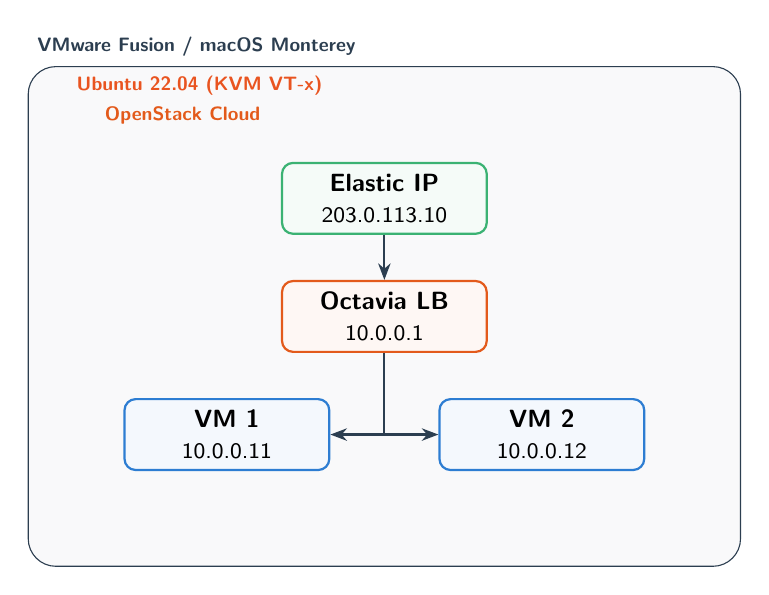
\begin{tikzpicture}[
    font=\small,
    box/.style={draw=#1, fill=#1!5, thick, rounded corners=4pt, minimum width=2.6cm, minimum height=0.9cm, align=center},
    arr/.style={-{Stealth[length=6pt]}, thick, color=macos},
]
\node[box=osgreen] (eip) at (0,0) {\textbf{Elastic IP} \\ \footnotesize 203.0.113.10};
\node[box=osaccent] (lb) at (0,-1.5) {\textbf{Octavia LB} \\ \footnotesize 10.0.0.1};
\node[box=osblue] (vm1) at (-2,-3) {\textbf{VM 1} \\ \footnotesize 10.0.0.11};
\node[box=osblue] (vm2) at (2,-3) {\textbf{VM 2} \\ \footnotesize 10.0.0.12};
\draw[arr] (eip) -- (lb);
\draw[arr] (lb) |- (vm1);
\draw[arr] (lb) |- (vm2);
\begin{scope}[on background layer]
    \node[draw=osaccent, dashed, rounded corners=6pt, fill=osaccent!2, fit=(lb)(vm1)(vm2)(eip), inner sep=10pt] (os) {};
    \node[draw=ubuntu, dashed, rounded corners=8pt, fill=ubuntu!2, fit=(os), inner sep=10pt] (ub) {};
    \node[draw=macos, rounded corners=10pt, fill=macos!3, fit=(ub), inner sep=14pt] (mac) {};
    \node[color=osaccent, font=\bfseries\scriptsize, anchor=south west] at (os.north west) {OpenStack Cloud};
    \node[color=ubuntu, font=\bfseries\scriptsize, anchor=south west] at (ub.north west) {Ubuntu 22.04 (KVM VT-x)};
    \node[color=macos, font=\bfseries\scriptsize, anchor=south west] at (mac.north west) {VMware Fusion / macOS Monterey};
\end{scope}
\end{tikzpicture}
\end{center}

\vspace{0.2em}
\textit{Note: this Octavia LBaaS branch was later abandoned in favour of a manual HAProxy VM. Octavia setup proved unreliable in DevStack without significant extra configuration.}

\section*{3. Research OpenStack Components}
\begin{itemize}
    \item \textbf{Nova} --- Compute service managing VM lifecycles via the KVM hypervisor.
    \item \textbf{Keystone} --- Identity service handling authentication, authorization, and trusts.
    \item \textbf{Ceilometer} --- Telemetry agent; polls hypervisor/Nova for resource usage and publishes samples.
    \item \textbf{Gnocchi} --- Time-series metric database; stores samples under per-resource archive policies.
    \item \textbf{Aodh} --- Alarm evaluation service; queries Gnocchi and fires actions when a threshold is crossed.
    \item \textbf{Heat} --- Orchestration engine; reads HOT templates and creates/destroys resources in response to signals.
\end{itemize}

\section*{4. Environment Setup}
Migrated to Ubuntu 24.04 LTS via VirtualBox to comply with DevStack's modern Python requirements.
\begin{enumerate}
    \item Forced nested KVM VT-x: \texttt{VBoxManage modifyvm "openStack" --nested-hw-virt on}
    \item Bridged VirtualBox networking to the host to avoid MAC filtering drops.
    \item Cloned DevStack, configured \texttt{local.conf}, executed \texttt{./stack.sh}.
\end{enumerate}

\section*{5. Target Architecture}
The static pair was replaced by a dynamic pool managed by a closed telemetry/orchestration loop, scaling strictly on CPU utilization.

\vspace{0.5em}
\begin{center}
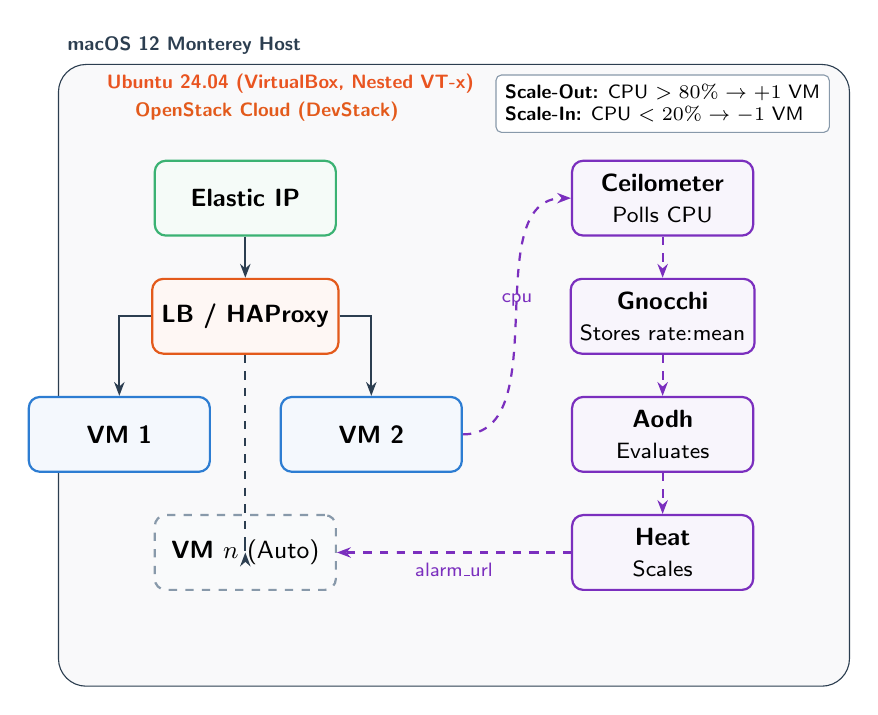
\begin{tikzpicture}[
    font=\small,
    box/.style={draw=#1, fill=#1!5, thick, rounded corners=4pt, minimum width=2.3cm, minimum height=0.95cm, align=center},
    arr/.style={-{Stealth[length=5pt]}, thick, color=macos},
    sig/.style={-{Stealth[length=5pt]}, dashed, thick, color=ospurple},
]
\node[box=osgreen] (eip) at (0,1.2) {\textbf{Elastic IP}};
\node[box=osaccent] (lb) at (0,-0.3) {\textbf{LB / HAProxy}};
\node[box=osblue] (vm1) at (-1.6,-1.8) {\textbf{VM 1}};
\node[box=osblue] (vm2) at (1.6,-1.8) {\textbf{VM 2}};
\node[box=osgray, dashed] (vm3) at (0,-3.3) {\textbf{VM $n$}\ (Auto)};

\node[box=ospurple] (ceil) at (5.3, 1.2)  {\textbf{Ceilometer} \\ \footnotesize Polls CPU};
\node[box=ospurple] (gno)  at (5.3, -0.3) {\textbf{Gnocchi} \\ \footnotesize Stores rate:mean};
\node[box=ospurple] (aodh) at (5.3, -1.8) {\textbf{Aodh} \\ \footnotesize Evaluates};
\node[box=ospurple] (heat) at (5.3, -3.3) {\textbf{Heat} \\ \footnotesize Scales};

\draw[arr] (eip) -- (lb);
\draw[arr] (lb) -| (vm1);
\draw[arr] (lb) -| (vm2);
\draw[arr, dashed] (lb) |- (vm3);

\draw[sig] (vm2.east) .. controls +(1.2,0) and +(-1.2,0) .. (ceil.west) node[midway, above, font=\scriptsize] {cpu};
\draw[sig] (ceil) -- (gno);
\draw[sig] (gno) -- (aodh);
\draw[sig] (aodh) -- (heat);
\draw[sig] (heat.west) .. controls +(-1.2,0) and +(1.2,0) .. (vm3.east) node[midway, below, font=\scriptsize] {alarm\_url};

\node[draw=osgray, fill=white, rounded corners=2pt, font=\scriptsize, align=left, minimum width=3.6cm] at (5.3, 2.4) {
    \textbf{Scale-Out:} CPU $> 80\% \rightarrow +1$ VM \\
    \textbf{Scale-In:} CPU $< 20\% \rightarrow -1$ VM
};

\begin{scope}[on background layer]
    \node[draw=osaccent, dashed, rounded corners=6pt, fill=osaccent!2, fit=(eip)(vm3)(ceil)(heat), inner sep=10pt] (os2) {};
    \node[draw=ubuntu, dashed, rounded corners=8pt, fill=ubuntu!2, fit=(os2), inner sep=10pt] (ub2) {};
    \node[draw=macos, rounded corners=10pt, fill=macos!3, fit=(ub2), inner sep=14pt] (mac2) {};
    \node[color=osaccent, font=\bfseries\scriptsize, anchor=south west] at (os2.north west) {OpenStack Cloud (DevStack)};
    \node[color=ubuntu, font=\bfseries\scriptsize, anchor=south west] at (ub2.north west) {Ubuntu 24.04 (VirtualBox, Nested VT-x)};
    \node[color=macos, font=\bfseries\scriptsize, anchor=south west] at (mac2.north west) {macOS 12 Monterey Host};
\end{scope}
\end{tikzpicture}
\end{center}

\section*{6. The Bugs Encountered}

\subsection*{Bug --- \texttt{signal\_url} vs \texttt{alarm\_url} (root cause of all 401s)}
\begin{bugbox}{Every alarm action returned \texttt{401 Unauthorized}}
\texttt{OS::Heat::ScalingPolicy} exposes two different attributes:
\begin{itemize}
    \item \texttt{signal\_url} --- requires a valid Keystone token.
    \item \texttt{alarm\_url} --- pre-signed, no token required.
\end{itemize}
The template used \texttt{signal\_url} throughout. Aodh's notifier correctly fired on every threshold breach but every HTTP POST bounced with \texttt{401} because Aodh does not attach a bearer token to webhook calls. The stack's trust and Aodh's service-user credentials both verified correct independently, making this bug resistant to diagnosis.
\end{bugbox}
\begin{fixbox}{Swap the attribute}
\begin{lstlisting}
alarm_actions:
  - { get_attr: [scale_out_policy, alarm_url] }   # not signal_url
\end{lstlisting}
Confirmed via \texttt{openstack orchestration resource type show OS::Heat::ScalingPolicy}. After the swap, manual \texttt{curl -X POST \$ALARM\_URL} returned \texttt{200 OK} with no \texttt{Authorization} header, and Aodh-triggered scale-outs began provisioning VMs automatically.
\end{fixbox}
\newpage
\section*{7. Final Working Heat Template}
\begin{lstlisting}
heat_template_version: 2021-04-16
description: Auto-scaling CirrOS instances on CPU thresholds (validated working config).

resources:

  web_server_group:
    type: OS::Heat::AutoScalingGroup
    properties:
      min_size: 1
      max_size: 3
      resource:
        type: OS::Nova::Server
        properties:
          flavor: m1.tiny
          image: cirros-0.6.3-x86_64-disk
          networks:
            - network: private
          metadata:
            server_group: { get_param: "OS::stack_id" }

  scale_out_policy:
    type: OS::Heat::ScalingPolicy
    properties:
      adjustment_type: change_in_capacity
      auto_scaling_group_id: { get_resource: web_server_group }
      scaling_adjustment: 1
      cooldown: 120

  scale_in_policy:
    type: OS::Heat::ScalingPolicy
    properties:
      adjustment_type: change_in_capacity
      auto_scaling_group_id: { get_resource: web_server_group }
      scaling_adjustment: -1
      cooldown: 180

  cpu_alarm_high:
    type: OS::Aodh::GnocchiAggregationByResourcesAlarm
    properties:
      description: "Scale OUT - CPU > 80%"
      metric: cpu
      aggregation_method: rate:mean
      granularity: 300
      evaluation_periods: 1
      threshold: 800000000
      comparison_operator: gt
      resource_type: instance
      query:
        str_replace:
          template: '{"=": {"server_group": "STACK_ID"}}'
          params:
            STACK_ID: { get_param: "OS::stack_id" }
      alarm_actions:
        - { get_attr: [scale_out_policy, alarm_url] }

  cpu_alarm_low:
    type: OS::Aodh::GnocchiAggregationByResourcesAlarm
    properties:
      description: "Scale IN - CPU < 20%"
      metric: cpu
      aggregation_method: rate:mean
      granularity: 300
      evaluation_periods: 1
      threshold: 200000000
      comparison_operator: lt
      resource_type: instance
      query:
        str_replace:
          template: '{"=": {"server_group": "STACK_ID"}}'
          params:
            STACK_ID: { get_param: "OS::stack_id" }
      alarm_actions:
        - { get_attr: [scale_in_policy, alarm_url] }

outputs:
  scale_out_url:
    value: { get_attr: [scale_out_policy, alarm_url] }
  scale_in_url:
    value: { get_attr: [scale_in_policy, alarm_url] }
\end{lstlisting}

\section*{8. Required One-Time Environment Fix}
\begin{lstlisting}
openstack metric archive-policy-rule create \
  --archive-policy-name ceilometer-low-rate \
  --metric-pattern "cpu" \
  cpu-rate-rule
\end{lstlisting}

\section*{9. Required Per-Deployment Manual Step}
\begin{lstlisting}
STACK_ID=$(openstack stack show karimTest -c id -f value)
for VM_ID in $(openstack server list -f value -c ID); do
  openstack metric resource update --type instance \
    --attribute server_group:"$STACK_ID" $VM_ID
done
\end{lstlisting}

\section*{10. Verification Sequence}
\begin{enumerate}
    \item \texttt{openstack metric archive-policy-rule list} --- confirm \texttt{cpu-rate-rule} present.
    \item \texttt{openstack stack create -t autoscale.yaml karimTest} $\to$ wait for \texttt{CREATE\_COMPLETE}.
    \item Patch \texttt{server\_group} on the spawned VM(s) (Section 9).
    \item \texttt{openstack metric measures show <cpu\_uuid> --aggregation rate:mean} --- confirm non-empty after one 5-min cycle.
    \item \texttt{openstack alarm list} --- confirm state moves from \texttt{insufficient data} to \texttt{ok}.
    \item Generate real CPU load on a VM console, confirm \texttt{cpu\_alarm\_high} $\to$ \texttt{alarm} and a new VM is provisioned.
    \item Confirm \texttt{alarm\_url} returns \texttt{200 OK} with no \texttt{Authorization} header on manual \texttt{curl} test.
    \item Stop load, wait for \texttt{cpu\_alarm\_low} $\to$ \texttt{alarm}, confirm scale-in deletes a VM back toward \texttt{min\_size}.
\end{enumerate}

\section*{11. Outcome}
End-to-end closed-loop autoscaling validated on CirrOS/\texttt{m1.tiny} under DevStack \texttt{2024.1}: Ceilometer polling $\to$ Gnocchi \texttt{rate:mean} storage $\to$ Aodh threshold evaluation $\to$ Heat \texttt{alarm\_url}-triggered scale-out/scale-in, both directions independently confirmed under real and synthetic CPU load.

\end{document}